\begin{solution}{normal}
We have a meniscus as shown in figure, and separate a
fraction of water (depicted in grey) by a fictitious horizontal plane passing the flat bottom of the meniscus, and consider the force balance for the grey volume. At the
separation plane inside the liquid, the hydrostatic pressure
equals to the atmospheric one. Indeed, at the bottom of
the meniscus, through the flat water-air interface, there is
no capillary pressure, hence the hydrostatic gauge pressure
must be zero; inside the liquid, the hydrostatic pressure is
a function of height only, so the pressure remains equal
to the atmospheric one through the horizontal plane. So,
the volume depicted by grey in the figure is surrounded by
atmospheric pressure, i.e. there is no extra net force acting
on it due to pressure.
\begin{center}
    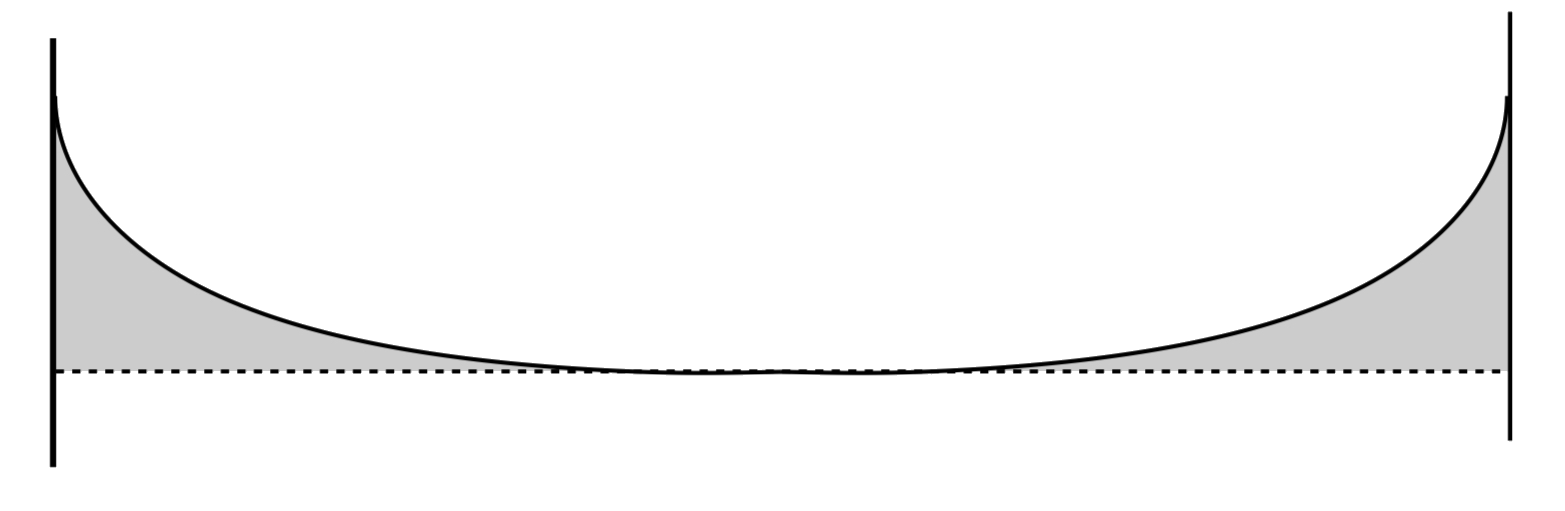
\includegraphics[width=8cm]{pr26.png}
\end{center}
By idea 17, the  gauge pressure due to capillary forces across a curved interface is $\rho gh = \frac{\sigma}{r}$ in cylindrical geometry where $H=V/(\pi r^2)$ gives the radius of the cylinder. We can determine the volume through a force balance:
$$\rho \Delta Vg=\sigma (2\pi r)$$
Plugging in our expression for $r$ gives:
$$\Delta V = \frac{2\sigma}{\rho g}\sqrt{\frac{V\pi}{H}} \approx 0.59 \text{ mL}$$
\blfootnote{It is believed that the symbolic answer to this problem in the handout is incorrect as it is not dimensionally correct.}
\end{solution}